\documentclass[12pt, oneside]{article}

\usepackage[letterpaper, scale=0.8, centering]{geometry}
\usepackage{fancyhdr}
\setlength{\parindent}{0em}
\setlength{\parskip}{1em}

\pagestyle{fancy}
\fancyhf{}
\renewcommand{\headrulewidth}{0pt}
\rfoot{{\footnotesize Copyright Mia Minnes, 2025, Version \today~(\thepage)}}

\usepackage{titlesec}

\author{CSE105W25}

\newcommand{\instructions}{{\bf For all HW assignments:} Weekly homework 
may be done individually or in groups of up to 3 students. 
You may switch HW partners for different HW assignments. 
Please ensure your name(s) and PID(s) are clearly visible on the first page of your homework submission 
and then upload the PDF to Gradescope. If working in a group, submit only one submission per group: 
one partner uploads the submission through their Gradescope account and then adds the other group member(s) 
to the Gradescope submission by selecting their name(s) in the ``Add Group Members" dialog box. 
You will need to re-add your group member(s) every time you resubmit a new version of your assignment.
 Each homework question will be graded either for correctness (including clear and precise explanations and 
 justifications of all answers) or fair effort completeness. 
 On the ``graded for correctness"
 questions, you may only collaborate with CSE 105 students in your group; if your
 group has questions about a problem, you may ask in drop-in help hours or post a private
post (visible only to the Instructors) on Piazza. On the "graded for completeness" questions, you 
may collaborate with all other CSE 105 students this quarter, and you may make public posts about these questions 
on Piazza.

All submitted homework for this class must be typed. 
You can use a word processing editor if you like (Microsoft Word, Open Office, Notepad, Vim, Google Docs, etc.) 
but you might find it useful to take this opportunity to learn LaTeX. 
LaTeX is a markup language used widely in computer science and mathematics. 
The homework assignments are typed using LaTeX and you can use the source files 
as templates for typesetting your solutions.
To generate state diagrams of machines, you can (1) use the LaTex tikzpicture
environment (see templates in the class notes), or (2) use the software tools Flap.js or
JFLAP described in the class syllabus (and include a screenshot in your PDF), or (3) you can carefully
and clearly hand-draw
the diagram and take a picture and include it in your PDF.
We recommend that you
submit early drafts to Gradescope so that in case of any technical difficulties, at least some of your
work is present. You may update your submission as many times as you'd like up to the deadline.


{\bf Integrity reminders}
\begin{itemize}
\item Problems should be solved together, not divided up between the partners. The homework is
designed to give you practice with the main concepts and techniques of the course, 
while getting to know and learn from your classmates.
\item On the "graded for correctness"
questions, you may only collaborate with CSE 105 students in your group.
You may ask questions about the homework in office hours (of the instructor, TAs, and/or tutors) and 
on Piazza (as private notes viewable only to the Instructors).  
You \emph{cannot} use any online resources about the course content other than the class material 
from this quarter -- this is primarily to ensure that we all use consistent notation and
definitions (aligned with the textbook) and also to protect the learning experience you will have when
the `aha' moments of solving the problem authentically happen.
\item Do not share written solutions or partial solutions for homework with 
other students in the class who are not in your group. Doing so would dilute their learning 
experience and detract from their success in the class.
\end{itemize}

}

\newcommand{\gradeCorrect}{({\it Graded for correctness}) }
\newcommand{\gradeCorrectFirst}{\gradeCorrect\footnote{This means your solution 
will be evaluated not only on the correctness of your answers, but on your ability
to present your ideas clearly and logically. You should explain how you 
arrived at your conclusions, using
mathematically sound reasoning. Whether you use formal proof techniques or 
write a more informal argument
for why something is true, your answers should always be well-supported. 
Your goal should be to convince the
reader that your results and methods are sound.} }
\newcommand{\gradeComplete}{({\it Graded for completeness}) }
\newcommand{\gradeCompleteFirst}{\gradeComplete\footnote{This means you will 
get full credit so long as your submission demonstrates honest effort to 
answer the question. You will not be penalized for incorrect answers. 
To demonstrate your honest effort in answering the question, we 
expect you to include your attempt to answer *each* part of the question. 
If you get stuck with your attempt, you can still demonstrate 
your effort by explaining where you got stuck and what 
you did to try to get unstuck.} }

\usepackage{tikz}
\usetikzlibrary{automata,positioning,arrows}

\input{../../resources/discrete-math-packages}

\newcommand{\SUBSTRING}{\textsc{Substring}}
\newcommand{\REP}{\textsc{Rep}}
\newcommand{\blank}{\scalebox{1.5}{\textvisiblespace}}

\titleformat{\subsubsection}[runin]
   {\normalfont\bfseries}{}{}{}
   
\title{ProjectCSE105W25: Project}
\date{Due March 19, 2025 at 8am}

\begin{document}
\maketitle

\thispagestyle{fancy}


\vspace{-20pt}

The CSE 105 project is designed for you to go deeper and 
extend your work on assignments 
and to see how some of the abstract notions we discuss can 
be implemented in concrete ways. 
The project is an individual assignment and has two tasks: 

Task 1: Checking the consistency of two regular properties, and

\vspace{-15pt}

Task 2: Illustrating a mapping reduction

In each task, you'll be implementing some of the theoretical concepts we've talked about in a programming language of your choosing, and then presenting your reasoning and demonstrating your code. Getting practice with this 
style of presentation is a good thing  for you to learn in general and a rich 
way for us to assess your skills. 

\vspace{-20pt}

\subsubsection*{What resources can you use?} This project must be completed individually, 
without any help from other people, including the course staff (other than logistics support if 
you get stuck with screencast). You should be the architect of your approach to the project.
You can refer to any of this quarter's CSE 105 offering (notes, readings, class videos, homework feedback). 
Tools for drawing state diagrams (like Flap.js and JFLAP and the PrairieLearn automata library) can be used to help draw the diagrams 
in the project too. However, do not copy / screenshot material that was not produced by you directly to your project writeup. Instead, you can refer to it in your own words and include a citation to the resource you referenced.

These resources should be more than enough.
If you are struggling to get started and want to look elsewhere online, 
you must acknowledge this by listing and citing any resources you consult 
(even if you do not explicitly quote them), including any large-language model style resources (ChatGPT, Bard, Co-Pilot, etc.). 
Link directly to them and include the name of the author / video creator, 
any and all search strings or prompts you used, and the reason you consulted this reference.  Also, a word of caution, make sure you validate and check 
any code produced by these aids. Last quarter there were a lot of examples
of project submissions that fed the prompt of the project 
directly to a LLM code  generator and got wrong implementations back.

{\bf Submitting the project} You will submit a PDF plus a video file (.mp4) for each. All file submissions will be in Gradescope. Upload the four files themselves. It is your responsibility to ensure that the files are playable within Gradescope. No Google Drive links, YouTube links, or .mov files.

\newpage
\subsubsection*{Your videos:} You may produce screencasts 
with any software you choose. 
One option is to record yourself with Zoom; a tutorial on how to use 
Zoom to record a 
screencast (courtesy of Prof. Joe Politz)  is here: 

\url{https://drive.google.com/open?id=1KROMAQuTCk40zwrEFotlYSJJQdcG_GUU}.

The video that was produced from that recording session in Zoom is here:

\url{https://drive.google.com/open?id=1MxJN6CQcXqIbOekDYMxjh7mTt1TyRVMl}

Please send an email to the instructor 
(minnes@ucsd.edu) if you have 
concerns about  the video / screencast components of this project or 
cannot complete projects in this style for some reason.

\vspace{-20pt}

\subsubsection*{Task 1: Checking the consistency of two regular properties}

When we have a list of desired properties, it's helpful to know whether there 
are any examples that satisfy *all* of them at once; 
in other words, whether the  properties are 
consistent with each other. For example, the properties of 
a string starting with $0$ and a string starting with $1$ are {\it not} consistent, 
because there isn't any example of a string that simultaneously starts with $0$ and with $1$.
In this part of the 
project, you'll use the decidability of the emptiness problem for DFA to 
build an algorithm that checks if two given regular properties are consistent.

Specifically:

\vspace{-20pt}

\begin{enumerate}
\item Write a program in Java, Python, JavaScript, C++ , or another programming language of your choosing that checks the consistency of two arbitrary regular properties.  The function input must be a {\bf pair of strings} and part of your work in this program  is to design string representations for any arbitrary DFA since those DFAs will be how you represent the properties. The function output must be a {\bf boolean}:
true (if the pair of strings represent consistent regular properties) or 
false (if the pair of strings do not represent consistent regular properties).
\begin{itemize}
   \item You might find it useful to use the algorithm for building a DFA that recognizes the {\bf intersection} of the languages of two DFA and the algorithm for testing the {\bf emptiness} of the language of a DFA.
   \item One test case for your program is the following: Consider the DFA $M_0$ and $M_1$ 

   \begin{tabular}{cc}
      $M_0$& $M_1$ \\
      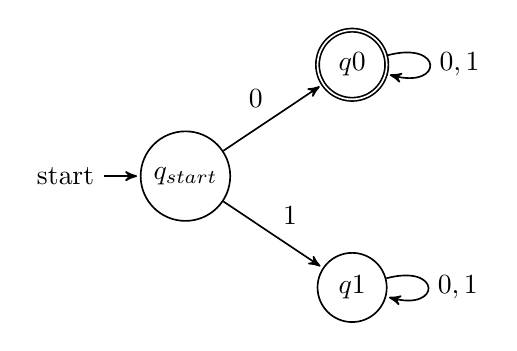
\begin{tikzpicture}[->,>=stealth',shorten >=1pt, auto, node distance=2cm, semithick]
         \tikzstyle{every state}=[text=black, fill=none]
         
         \node[initial,state] (qs)          {$q_{start}$};
         \node[state,accepting]    (q0) [above right of=qs, xshift=20pt] {$q0$};
         \node[state]         (q1) [below right of=qs, xshift=20pt] {$q1$};
         
         \path (qs) edge  [bend left=0] node {$0$} (q0)
             (q0) edge [loop right] node {$0,1$} (q0)
             (qs) edge [bend left=0] node {$1$} (q1)
             (q1) edge [loop right] node {$0,1$} (q1)
         ;
      \end{tikzpicture}&
      \begin{tikzpicture}[->,>=stealth',shorten >=1pt, auto, node distance=2cm, semithick]
         \tikzstyle{every state}=[text=black, fill=none]
         
         \node[initial,state] (rs)          {$r_{start}$};
         \node[state]    (r0) [above right of=qs, xshift=20pt] {$r0$};
         \node[state,accepting]         (r1) [below right of=qs, xshift=20pt] {$r1$};
         
         \path (rs) edge  [bend left=0] node {$0$} (r0)
             (r0) edge [loop right] node {$0,1$} (r0)
             (rs) edge [bend left=0] node {$1$} (r1)
             (r1) edge [loop right] node {$0,1$} (r1)
         ;
      \end{tikzpicture}
   \end{tabular}

   and let $w_0$ be the string representing $M_0$ and let $w_1$ be the string representing $M_1$. Then the result of your program on the input $w_0, w_1$ 
   should be {\bf false} because the properties represented by $M_0$ and $M_1$ 
   are inconsistent.\footnote{To see why, notice that $L(M_0)$ is the set of strings that start with $0$ and $L(M_1)$ is the set of strings that start with $1$.}
   \item The algorithm you implement needs to work with any pair of strings given as input (you should first parse each string in the input to see if it is formatted to represent a DFA). Your explanation of the algorithm should be such that most programmers can replicate the algorithm correctly. If you would like, you may use aids such as co-pilot or ChatGPT to help you write this program. 
   However, you should test the code that is produced and be able to explain what it is doing. Your code needs to be well-organized and well-documented.
   As a header in your code file or as an appendix in your PDF submission, include a comment block describing any resources that were used to 
   help generate your code, including any and all prompts used in interactions 
   with LLM coding tools.
\end{itemize}
\item To demonstrate your program, you will show how it runs (at least) twice: once with the test input $w_0, w_1$ described above, and once with test input $x_0, x_1$ that you define to demonstrate when the program outputs {\bf true}. Your choice of $x_0, x_1$ needs to satisfy the following conditions:
\begin{itemize}
\item $x_0$ and $x_1$ each represent DFA over the same fixed alphabet, 
\item the DFA represented by $x_0$ and $x_1$ do not recognize the same language,
\item the DFA represented by $x_0$ and $x_1$ do not recognize the empty set or the set of all strings or the set of all strings starting with $0$ or the set of all strings starting with $1$.
\end{itemize}  
As part of your demonstration, describe your choice of $x_0$ and $x_1$, clearly 
specifying the DFAs they represent and the languages recognized by these DFAs.
Each demo run of the program should include: 
\begin{itemize}
\item Side-by-side view of an English / mathematical formulation of the properties and DFA corresponding to the demo run, along with their string representation as input strings to the program.
\item Talk-aloud trace of the running of your program on the input pair of strings representing the two properties for the demo. During the trace, talk about the software design choices you made
(e.g. which data structures are you using, etc.) and how they impact the program. Also, give credit to any resources you used to make these design choices or develop the code. 
\item Recording of actually running your program on the input pair of strings for this demo, including interpreting the output the program gives and connecting it to whether the properties represented by the input are consistent or not.
\end{itemize}
\end{enumerate}

\newpage 

{\bf Checklist for submission} For this task, you will submit a PDF file plus a 3-5 minute video.


\begin{itemize}
   \item[(PDF)] Submit a single PDF file that clearly describes the design choices you made, includes
   all relevant code, and includes all relevant information (definition, representation, justification) about the examples used to demonstrate your program and screenshots from running your program on the examples. The writeup should use precise language and notation for all terms and clearly communicate the goal and approach of your program.
   \item[(PDF)] The documentation for your program should include a description of how input strings are parsed to represent DFA, in general and for the specific examples of $w_0, w_1, x_0, x_1$.
   \item[(Video)] The video should start with your face and your student ID visible for a few seconds at the beginning, and introduce yourself audibly while on screen. You don't have to be on camera for the  rest of the video, though it's fine if you are. We are looking for a brief confirmation that  it's you creating the video and doing the work you submitted.
\item[(Video)] The video includes the full program demo twice (once with the input $w_0,w_1$ and once with the input $x_0,x_1$), and includes the 
a mathematical and/or English definition of the regular properties you are using, connected to their
representations as strings when input to the program, and the talk-aloud trace of running the program on these inputs and its output connecting back to the notion of consistency of regular properties.
\end{itemize}

{\bf Note}: Clarity and brevity are both important aspects of your video.  In previous years, we've seen 
students speed up their videos to get below the 5 minute upper bound. This is ok so long as it doesn't 
compromise clarity. If the graders need to slow your video down to understand
it, it may not earn full credit.



{\bf Possible extensions}: If you're enjoying working on this and want to go deeper, here are a few additions you can consider. You will not be graded on any of these, and you should still make sure your project has the core functionality described above, but these extensions give you an opportunity to explore further.
\begin{itemize}
   \item Build a preprocesing step so that the regular properties can be expressed using NFA or regular expressions (in addition to DFA). You'll need to think about how to represent NFA and/or regular expressions as strings, and then how to convert them to DFA.
   \item Extend your work so that your program can test for consistency of more than two regular properties.
\end{itemize}

\newpage
\subsubsection*{Task 2: Illustrating a mapping reduction}

We can use mapping reductions to prove that interesting computational 
problems are undecidable, building on 
the undecidability of other computational problems.
In this part of the project, you'll choose a specific {\bf mapping reduction}
from an undecidable language of your choice to 
$$EQ_{TM} = \{ \langle M_1, M_2 \rangle \mid M_1, M_2 \text{ are Turing machines and } L(M_1) = L(M_2) \}$$
and implement a computable function that witnesses it
using a  programming language of your choice (aka a high-level description of a Turing machine that computes it).
You will then demonstrate  how your construction works for some test examples.

Specifically:

\vspace{-20pt}

\begin{enumerate}
\item Choose an undecidable language (other than $EQ_{TM}$) that 
we discussed in class or in the homework
or in review quizzes or in the textbook . {\it Note:
if you'd like to consider an undecidable language we have not discussed instead, 
please check with Prof. Minnes first. 
You must do so no later than the start of Week 10.}
\item Write a program in Java, Python, JavaScript, C++ , or another programming language of your choosing that implements a computable function witnessing this mapping reduction.  The function input must be a {\bf string}  and the function 
output must be a {\bf string}. Part of your work in this program 
is to design string representations for arbitrary instances of the model of 
computation the computational problems being compared in the mapping reduction.
\begin{itemize}
   \item You may use our class material for ideas on the algorithm that your program will implement. The algorithm you implement needs to be general enough to decide whether each input string is in the language or not. Your explanation of the algorithm should be such that most programmers can replicate the algorithm correctly.
   \item If you would like, you may use aids such as co-pilot or ChatGPT to help you write this program. 
   However, you should test the code that is produced and be able to explain what it is doing. Your code needs to be well-organized and well-documented.
   As a header in your code file or as an appendix in your PDF submission, include a comment block describing any resources that were used to 
   help generate your code, including any and all prompts used in interactions 
   with LLM coding tools.
\end{itemize}

\item To demonstrate your program, you will need to run it for an example positive and negative instance. That is to say, if you are implementing 
a computable function witnessing $X \leq_m EQ_{TM}$, you will select one string that is in $X$ and one string that is not in $X$, and you will 
 demonstrate running your program on each of these strings and explain why 
 the output of the function is good.
\end{enumerate}

\newpage

{\bf Checklist for submission} For this task, you will submit a PDF file plus a 3-5 minute video.

\begin{itemize}
   \item[(PDF)] Submit a single PDF file that clearly describes the mapping reduction, including defining the undecidable language you 
   chose and the computable function that you will implement to witness its mapping reduction to $EQ_{TM}$, and includes all relevant code and documentation documentation for the program computing the function witnessing this mapping reduction. In particular, include a description of how input strings are parsed and how output strings correspond to input strings and a clear specification of your two example strings, explaining which is is a positive instance (and why) and which is a negative instance (and why not). The writeup should use precise language and notation for all terms and clearly communicate the goal and approach of your program.
   \item[(Video)] The video should start with your face and your student ID visible for a few seconds at the beginning, and introduce yourself audibly while on screen. You don't have to be on camera for the  rest of the video, though it's fine if you are. We are looking for a brief confirmation that  it's you creating the video and doing the work you submitted.
\item[(Video)] The video includes the mapping reduction you will be working with, and the 
example strings that you will be using, including explanations of why you chose this reduction and these strings (and why one of the strings is a positive instance and the other is a negative instance). The full program demo should be part of the video, with an explanation of the code and the software design choices you made and any resources you used, and then live screencasts running your code on each of your example inputs. 
Explain why the output of your program is what you would expect, by connecting the output of the 
program to the definition of the mapping reduction and your chosen parsing of input strings.
\end{itemize}

{\bf Note}: Clarity and brevity are both important aspects of your video.  In previous years, we've seen 
students speed up their videos to get below the 5 minute upper bound. This is ok so long as it doesn't 
compromise clarity. If the graders need to slow your video down to understand
it, it may not earn full credit.

\end{document}